\documentclass[aspectratio=169,12pt]{beamer}
\usepackage{amsmath}
\usepackage{amssymb}
\usepackage[most]{tcolorbox}
\usepackage{tikz}
\usepackage{graphicx}
\usepackage[sfdefault,lf]{FiraSans}
\renewcommand{\familydefault}{\sfdefault}
\setlength{\parindent}{0pt}
\everymath{\displaystyle}

\setbeamertemplate{navigation symbols}{}
\setbeamertemplate{footline}{}
\setbeamertemplate{headline}{}

\definecolor{mmpageWhite}{HTML}{FCFBF7}
\definecolor{mmtanSoft}{HTML}{F7F5EF}
\definecolor{mmgreenDeep}{HTML}{244B2C}
\definecolor{mmgreenLeaf}{HTML}{5D8A56}
\definecolor{mmgreenSoft}{HTML}{E4EFD9}
\definecolor{mmtext}{HTML}{163221}

\setbeamercolor{background canvas}{bg=mmpageWhite}
\setbeamercolor{normal text}{fg=mmtext,bg=mmpageWhite}

\newtcolorbox{MMProblemCard}[1][]{enhanced,breakable=false,colback=white,colframe=black,boxrule=1.5pt,arc=8pt,left=5pt,right=5pt,top=4pt,bottom=4pt,before skip=0pt,after skip=0pt,height=0.245\textheight,valign=top,#1}
\newcommand{\KoruIcon}{\raisebox{-0.2em}{
\includegraphics[height=1.05em]{../../SITE/header-logo.png}}}
\newcommand{\HoeIcon}{\raisebox{-0.2em}{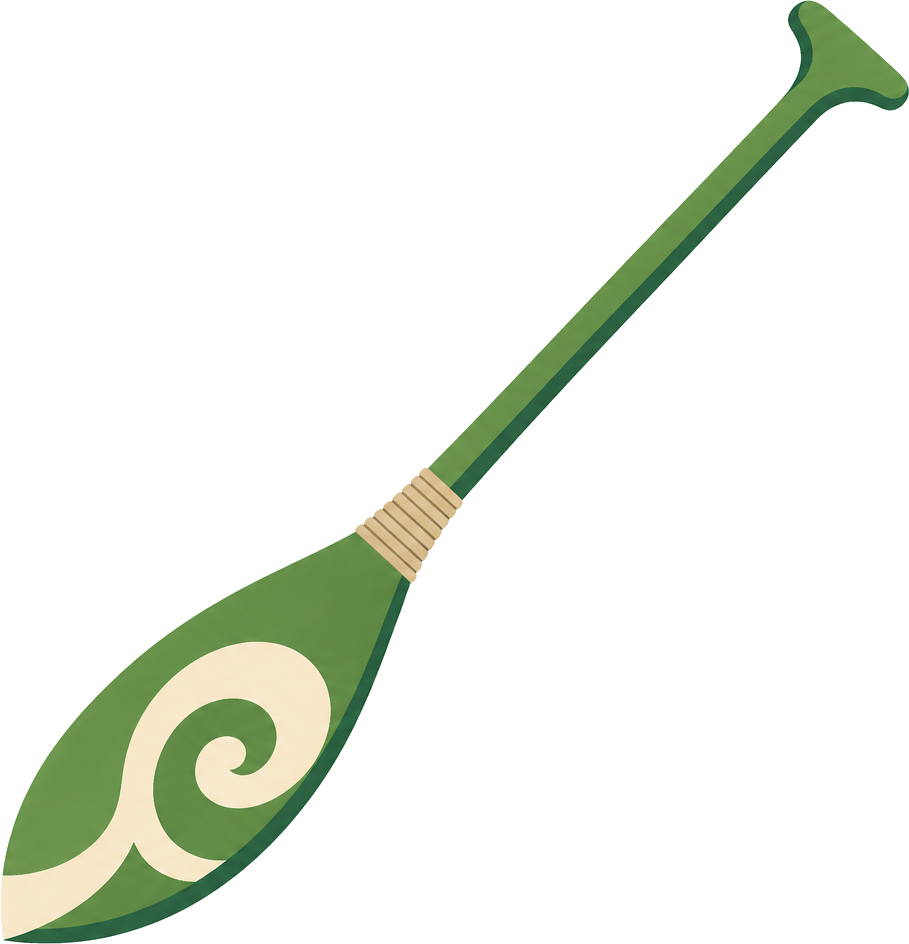
\includegraphics[height=1.05em]{../../SITE/hoe.png}}}
\newcommand{\ScaffoldIcons}[1]{\ifcase#1\or \HoeIcon\or \HoeIcon\hspace{0.22em}\KoruIcon\or \KoruIcon\hspace{0.22em}\KoruIcon\hspace{0.22em}\KoruIcon\fi}
\newcommand{\WorksheetTitle}[2]{%
  {\colorbox{mmtanSoft}{\parbox[c][2.0em][c]{0.975\linewidth}{%
    \hspace{0.25em}{\Large\bfseries\textcolor{mmgreenDeep}{#1}\hfill\ScaffoldIcons{#2}}}}
  \par\vspace{0.08em}{\color{mmgreenLeaf}\rule{\linewidth}{2.0pt}}\par\vspace{0.04em}}
}
\newcommand{\MMProblem}[2]{\begin{MMProblemCard}\raggedright\small\textbf{#1.} #2\par\end{MMProblemCard}}

\setbeamertemplate{background}{
 \begin{tikzpicture}[remember picture,overlay]
 \draw[black,line width=1.5pt,rounded corners=10pt]
 ([xshift=0.45cm,yshift=-0.45cm]current page.north west)
 rectangle
 ([xshift=-0.45cm,yshift=0.45cm]current page.south east);
 \end{tikzpicture}
}

% Default worksheet generation rules:
% use notes-style beamer pages
% use bordered cards for individual problems
% target 9 problems per frame in a 3x3 grid
% target 3 frames per scaffold by default where content allows

\begin{document}\begin{frame}[t]
\WorksheetTitle{Build Tasks}
\vspace{-0.18em}
\begin{columns}[T,onlytextwidth]
\begin{column}{0.32\textwidth}\MMProblem{1}{A rectangle is 12 cm by 6 cm with a semicircle of diameter 6 cm attached to one short side. Find the perimeter in terms of \mbox{$\pi$}.}\end{column}
\begin{column}{0.32\textwidth}\MMProblem{2}{A rectangle is 12 cm by 6 cm with a semicircle of diameter 6 cm attached to one short side. Find the area in terms of \mbox{$\pi$}.}\end{column}
\begin{column}{0.32\textwidth}\MMProblem{3}{A square of side 14 m has four quarter circles of radius 7 m drawn at the corners, making one full circle inside the square. Find the shaded area left inside the square but outside the circle. Give the exact answer in terms of \mbox{$\pi$}.}\end{column}
\end{columns}
\vspace{0.45em}
\begin{columns}[T,onlytextwidth]
\begin{column}{0.32\textwidth}\MMProblem{4}{A square of side 14 m has four quarter circles of radius 7 m drawn at the corners, making one full circle inside the square. Find the total curved length. Give the exact answer in terms of \mbox{$\pi$}.}\end{column}
\begin{column}{0.32\textwidth}\MMProblem{5}{A stadium shape has two straight sides of 18 cm and two semicircular ends of radius 4 cm. Find its perimeter in terms of \mbox{$\pi$}.}\end{column}
\begin{column}{0.32\textwidth}\MMProblem{6}{A stadium shape has two straight sides of 18 cm and two semicircular ends of radius 4 cm. Find its area in terms of \mbox{$\pi$}.}\end{column}
\end{columns}
\vspace{0.45em}
\begin{columns}[T,onlytextwidth]
\begin{column}{0.32\textwidth}\MMProblem{7}{A rectangle is 16 cm by 10 cm. A semicircle of diameter 10 cm is cut out from one short side. Find the remaining perimeter in terms of \mbox{$\pi$}.}\end{column}
\begin{column}{0.32\textwidth}\MMProblem{8}{A rectangle is 16 cm by 10 cm. A semicircle of diameter 10 cm is cut out from one short side. Find the remaining area in terms of \mbox{$\pi$}.}\end{column}
\begin{column}{0.32\textwidth}\MMProblem{9}{A square of side 12 cm has a quarter circle of radius 12 cm cut off from one corner. Find the perimeter of the remaining shape in terms of \mbox{$\pi$}.}\end{column}
\end{columns}
\end{frame}
\begin{frame}[t]
\WorksheetTitle{Build Tasks}
\vspace{-0.18em}
\begin{columns}[T,onlytextwidth]
\begin{column}{0.32\textwidth}\MMProblem{1}{A square of side 12 cm has a quarter circle of radius 12 cm cut off from one corner. Find the remaining area in terms of \mbox{$\pi$}.}\end{column}
\begin{column}{0.32\textwidth}\MMProblem{2}{A running track has two straight sections of 60 m and two semicircular ends of diameter 30 m. Find the total length of one lap in terms of \mbox{$\pi$}.}\end{column}
\begin{column}{0.32\textwidth}\MMProblem{3}{A running track has two straight sections of 60 m and two semicircular ends of diameter 30 m. Find the area enclosed by the inside edge in terms of \mbox{$\pi$}.}\end{column}
\end{columns}
\vspace{0.45em}
\begin{columns}[T,onlytextwidth]
\begin{column}{0.32\textwidth}\MMProblem{4}{}\end{column}
\begin{column}{0.32\textwidth}\MMProblem{5}{}\end{column}
\begin{column}{0.32\textwidth}\MMProblem{6}{}\end{column}
\end{columns}
\vspace{0.45em}
\begin{columns}[T,onlytextwidth]
\begin{column}{0.32\textwidth}\MMProblem{7}{}\end{column}
\begin{column}{0.32\textwidth}\MMProblem{8}{}\end{column}
\begin{column}{0.32\textwidth}\MMProblem{9}{}\end{column}
\end{columns}
\end{frame}
\end{document}
